\section{Introducción}

Considerando un frente de onda plano, el principio de construcción de
frentes de onda de Cristian Huyghens, dice que:
\begin{enumerate}
    \item Cada punto del frente de onda se constituye en un emisor
    isotrópico de ondas, esto para cualquier frente de onda.

    \item Los puntos de intersección de las ondas de estos emisores en
    un mismo tiempo, forman un nuevo frente de onda, mostrando cómo se
    propaga.
\end{enumerate}

Para visualizar esto, se mostrará el primer punto en un emisor
isotrópico, y el segundo, como se requiere un frente de onda plano, se
partirá de uno.

\begin{center}
    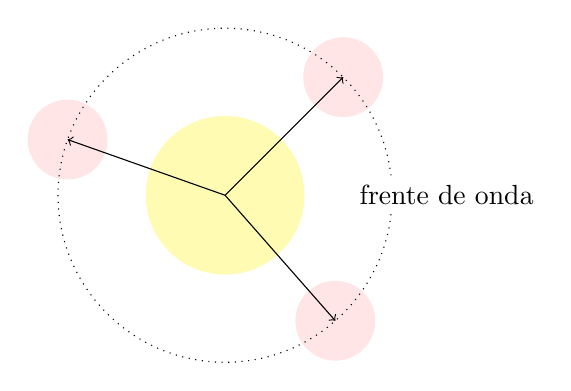
\begin{tikzpicture}
        % ~~~~ Circulos de los emisores ~~~~%
        \filldraw [color=yellow!30] (0,0) circle (1);
        \filldraw[color=red!10] (1.5,1.5) circle (0.5);
        \filldraw[color=red!10] (1.4,-1.59373775) circle (0.5);
        \filldraw[color=red!10] (-2,0.707106781) circle (0.5);

        % ~~~~~ Flechas de algunas de las ondas ~~~~%
        \draw[ -> ] (0,0) -- (1.5,1.5);
        \draw[ -> ] (0,0) -- (1.4,-1.59373775);
        \draw[ -> ] (0,0) -- (-2,0.707106781);

        % ~~~~ Frente de onda ~~~~%
        \draw[dotted] (0,0) circle (2.12132034) 
            node[xshift=80pt, fill=white] {frente de onda};
    \end{tikzpicture}
    \hspace{20pt}
    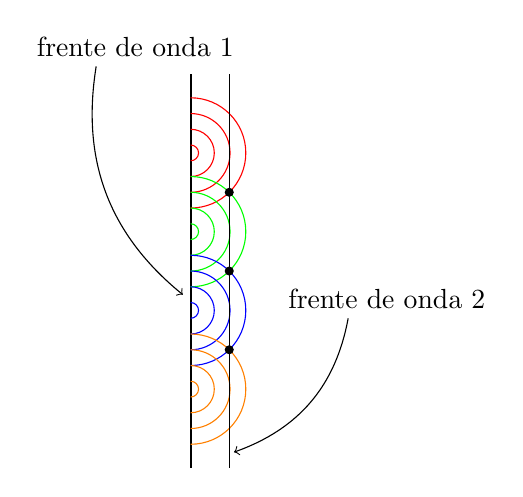
\begin{tikzpicture}
        \draw[thick] (0,-1.5) -- (0,3.5)
            node[yshift=10pt, xshift=-20pt] {frente de onda $1$};
        \draw[ -> ] (-1.2, 3.6) to [bend right] (-0.1, 0.7);

        
        % ~~~~ Emisores isotrópicos de algunos puntos ~~~~%
        \draw[red] (0,3.2) arc (90:-90:0.7);
        \draw[red] (0,3) arc (90:-90:0.5);
        \draw[red] (0,2.8) arc (90:-90:0.3);
        \draw[red] (0,2.6) arc (90:-90:0.1);

        \draw[green] (0,2.2) arc (90:-90:0.7);
        \draw[green] (0,2) arc (90:-90:0.5);
        \draw[green] (0,1.8) arc (90:-90:0.3);
        \draw[green] (0,1.6) arc (90:-90:0.1);

        \draw[blue] (0,1.2) arc (90:-90:0.7);
        \draw[blue] (0,1) arc (90:-90:0.5);
        \draw[blue] (0,0.8) arc (90:-90:0.3);
        \draw[blue] (0,0.6) arc (90:-90:0.1);

        \draw[orange] (0,0.2) arc (90:-90:0.7);
        \draw[orange] (0,0) arc (90:-90:0.5);
        \draw[orange] (0,-0.2) arc (90:-90:0.3);
        \draw[orange] (0,-0.4) arc (90:-90:0.1);

        % ~~~~ Nuevo frente de onda ~~~~%

        \filldraw (0.489897949,2) circle (0.05);
        \filldraw (0.489897949,1) circle (0.05);
        \filldraw (0.489897949,0) circle (0.05);
        
        \draw (0.489897949,3.5) -- (0.489897949,-1.5)
            node [midway, yshift=-10pt, xshift=20mm] {frente de onda $2$};
        \draw[ -> ] (2,0.4) to [bend left] (0.55, -1.3);
    \end{tikzpicture}
\end{center}